\documentclass[ima, 20pt, portrait, plainboxedsections]{sciposter}
%DIF LATEXDIFF DIFFERENCE FILE
%DIF DEL /Users/alhaddwt/Downloads/LaTeX_code_poster_poster.tex   Thu Aug  1 11:27:04 2019
%DIF ADD poster.tex                                               Thu Aug  1 11:24:20 2019

% Packages
\usepackage[english]{babel}
\usepackage[latin1]{inputenc}
\usepackage{times}
\usepackage{amsmath,amssymb}
\usepackage{multicol}
\usepackage{epstopdf}
\usepackage{graphicx}

\usepackage{color}
\usepackage{mathtools}
\usepackage{mathptmx}
\usepackage[11pt]{moresize}
\usepackage{wrapfig}
\usepackage{bbm}
\usepackage{xcolor}
\usepackage{tabularx}
\usepackage{bm}


% Commands
\newcommand{\ie}{\textit{i.e.}}
\newcommand{\eg}{\textit{e.g.}}
\newcommand{\cf}{\textit{cf.}}
\newcommand{\ud}{\mathrm{d}}
\newcommand{\prob}{\mathrm{P}}
\newcommand{\expt}{\mathrm{E}}
\newcommand{\var}{\mathrm{Var}}
\newcommand{\rset}{\mathbb{R}}
\newcommand{\nset}{\mathbb{N}}
\newcommand{\zset}{\mathbb{Z}}
\newcommand{\one}{\mathbf{1}}
\newcommand{\poisson}{\mathcal{P}}
\newcommand{\normal}{\mathcal{N}}
\newcommand{\binomial}{\mathcal{B}}
\newcommand{\Ordo}[1]{{\mathcal{O}}\left(#1\right)}
\newcommand{\ordo}[1]{{o}\left(#1\right)}
\newcommand{\red}[1]{{\color{red}#1}}
\newcommand{\blue}[1]{{\color{blue}#1}}
\newcommand{\green}[1]{{\color{green}#1}}
\renewcommand{\emph}{\red}

\newcommand{\R}{\mathbb{R}}
\newcommand{\E}{\mathbb{E}}
\newcommand{\N}{\mathbb{N}}
\newcommand{\Z}{\mathbb{Z}}
\newcommand{\V}{\mathbb{V}}
\newcommand{\Q}{\mathbb{Q}}
\newcommand{\K}{\mathbb{K}}
\newcommand{\C}{\mathbb{C}}
\newcommand{\T}{\mathbb{T}}
\newcommand{\I}{\mathbb{I}}

% Theorems
\newtheorem{Def}{Definition}
\newtheorem{Lem}{Lemma}
\newtheorem{Thm}{Theorem}

% Layout parameters
\newcommand{\imsize}{0.49\columnwidth}
%\definecolor{BoxCol}{rgb}{0,0,1}
\definecolor{BoxCol}{rgb}{0.9,0.4,0.4}
\definecolor{SectionCol}{rgb}{1,1,1}
\renewcommand{\titlesize}{\Huge}
\renewcommand{\sectionsize}{\Large}
\setmargins[2cm]


\leftlogo[1.3]{KAUST_Logo.pdf}  % KAUST LOGO
\rightlogo[1.3]{rwth.pdf}

% Overrides commands in sciposter.cls
%\setlength{\columnsep}{0.02\textheight}
%\setlength{\columnseprule}{0.001\textheight}
\setlength{\parskip}{0.002\textheight}

% Author info
\title{ On the Uncertainty of Wind Power Forecasts}
\author{ Waleed Alhaddad\textsuperscript{\textasteriskcentered} \qquad Ra\'ul  Tempone\textsuperscript{\textasteriskcentered}\textsuperscript{\textdagger}}
\institute{\textsuperscript{\textasteriskcentered}CEMSE Division, King Abdullah University of Science and Technology, Thuwal, Saudi Arabia \\ \textsuperscript{\textdagger}Alexander von Humboldt Professor in Mathematics of Uncertainty Quantification, RWTH Aachen University,  Germany}
%DIF PREAMBLE EXTENSION ADDED BY LATEXDIFF
%DIF UNDERLINE PREAMBLE %DIF PREAMBLE
\RequirePackage[normalem]{ulem} %DIF PREAMBLE
\RequirePackage{color}\definecolor{RED}{rgb}{1,0,0}\definecolor{BLUE}{rgb}{0,0,1} %DIF PREAMBLE
\providecommand{\DIFadd}[1]{{\protect\color{blue}\uwave{#1}}} %DIF PREAMBLE
\providecommand{\DIFdel}[1]{{\protect\color{red}\sout{#1}}}                      %DIF PREAMBLE
%DIF SAFE PREAMBLE %DIF PREAMBLE
\providecommand{\DIFaddbegin}{} %DIF PREAMBLE
\providecommand{\DIFaddend}{} %DIF PREAMBLE
\providecommand{\DIFdelbegin}{} %DIF PREAMBLE
\providecommand{\DIFdelend}{} %DIF PREAMBLE
%DIF FLOATSAFE PREAMBLE %DIF PREAMBLE
\providecommand{\DIFaddFL}[1]{\DIFadd{#1}} %DIF PREAMBLE
\providecommand{\DIFdelFL}[1]{\DIFdel{#1}} %DIF PREAMBLE
\providecommand{\DIFaddbeginFL}{} %DIF PREAMBLE
\providecommand{\DIFaddendFL}{} %DIF PREAMBLE
\providecommand{\DIFdelbeginFL}{} %DIF PREAMBLE
\providecommand{\DIFdelendFL}{} %DIF PREAMBLE
%DIF END PREAMBLE EXTENSION ADDED BY LATEXDIFF

\begin{document}
\newcommand{\ddd}[1]{\boldsymbol{#1}}
\renewcommand{\vec}[1]{\ddd{#1}}
\maketitle

%%% Begin of Multicols-Enviroment
\begin{multicols}{3}

\section*{Introduction}
Reliable wind power generation forecasting is crucial to:
 \begin{itemize} 
\item  Meet energy demand through renewable power sources.
\item  Energy trading of future excess power.
\item Design of Investment strategies.
 \end{itemize} 
We propose a parametric forecast error model to:
 \begin{itemize} 
\item  Simulate forecast error and quantify its uncertainty.
\item  Calibrate a forecast model for  optimal dispatch of electric power.
 \end{itemize} 
This model is based on:
 \begin{itemize} 
\item Parametric Stochastic Differential Equations.
\item Approximate Maximum Likelihood based on continuous optimization.
 \end{itemize} 
The result is a skewed stochastic process that simulates the uncertainty of wind power forecasts accounting for maximum power production limit and other temporal effects. We apply the model to historical Uruguayan data and forecasts (2016-2017).


\DIFaddbegin \section*{\DIFadd{Data}}

\DIFadd{To capture real-world performance of  wind power forecasts, our model incorporates historical wind power production data along with their corresponding forecasts.}\\

\DIFadd{We apply the model to Uruguayan wind power generation data and their corresponding numerical wind power production forecasts. }\\

\DIFadd{The wind power generation data set contains hourly samples of aggregated wind power production throughout the country. Each sample path contains 72 hourly observations and we have a total of 1217 sample paths spanning the year 2016 to 2017 (87,624 data points). }\\

\DIFadd{The numerical wind power generation forecast set contains  1217 forecasts of the wind power generation  corresponding to the actual  wind power generation data set mentioned above.
}

\begin{figure}[t]
\begin{center}
%DIF > \fbox{\rule{0pt}{2in} \rule{0.9\linewidth}{0pt}}
   %DIF > \includegraphics[width=0.8\linewidth]{Forecast_data_68.pdf}
    \includegraphics[width=0.8\linewidth]{Forecast_data_82.pdf}
\end{center}
   \caption{\DIFaddFL{Examples of wind power generation from the data set along with the wind power generation forecast.}}
\label{fig:long}
\label{fig:onecol}
\end{figure}

\DIFaddend \section*{Model}

\subsection*{Phenomenological  Model}

Let $X_t$ be the  wind power generation forecasts stochastic process defined by the  following parameterized stochastic differential equation (SDE),
\begin{equation}
\begin{split}
dX_t &= a(X_t; \bm{\theta}) dt + b (X_t; \bm{\theta} ) dW_t \quad t > 0 \\
X_0 & = X_0
\end{split}
\label{main}
\end{equation}

 \begin{itemize} 
%\item $\Delta_N$: any function of the number of samples, $N$. For example, $\Delta_N = \frac{1}{N}$.
\item $a(\cdot; \bm{\theta}):[0,1] \to \R $  a drift function.
\item $b (\cdot; \bm{\theta} ):[0,1] \to \R$  a  diffusion function.
\item $\bm{\theta}$: a vector of parameters.
\item $W_t$: Standard Wiener random process in $\R$.
 \end{itemize} 
%We prescribe the following derivative tracking model:
%\begin{itemize}
%\item $a(X_t; \bm{\theta})=  \dot{p}_t- \theta (X_t - p_t)$
%\item  $ b (X_t; \bm{\theta} )= \sqrt{2 \theta \alpha p_t(1-p_t) X_t (1-X_t)} $
%\end{itemize}
%where $p_t$ is the wind power forecast.

\subsection*{Physical Constrains}
Let $p_t$ be a numerical wind power forecast, which is an input to this approach. Then the model is given by the following It\^{o} stochastic differential equation,
\begin{equation}
\begin{split}
dX_t&= \dot{p} \ dt - \theta_t( X_t- p_t) \ dt + b (X_t; \bm{\theta} ) \ dW_t \quad t > 0 \\
X_0&=x_0
\end{split}
\end{equation}
As the  installed power production capacity is limited, we normalize with respect to the installation power. Thus our process must be limited to the range $[0,1]$. To enforce this constraint, we must have drift and diffusion control.
\subsubsection*{Diffusion\DIFdelbegin \DIFdel{Control}\DIFdelend : } The physical constraint is respected  by choosing  diffusion coefficient \DIFdelbegin \DIFdel{$ b (x; \bm{\theta} )= \sqrt{2 \theta_t \alpha p_t(1-p_t) x (1-x)} $ }\DIFdelend \DIFaddbegin \DIFadd{$ b (x; \bm{\theta} )= \sqrt{2 \theta_t \alpha x (1-x)} $ }\DIFaddend that is zero on the boundaries of $[0,1]$.
\subsubsection*{Drift\DIFdelbegin \DIFdel{Control}\DIFdelend : }
$X_t$ remains in $[0,1]$ a.s. by choosing $\theta_t$ as follows,
\begin{equation}
\theta_t = \max \left( \theta_0 \ , \ \frac{|\dot{p}_t|}{\min (p_t, 1-p_t)}  \right )
\end{equation}

\subsubsection*{Change of Variables:}
In order to avoid differentiation of the forecast $\dot{p}_t$ and simplify, we apply a change of variables \DIFdelbegin \begin{displaymath}\DIFdel{V_t = X_t - p_t}\end{displaymath}  %DIFAUXCMD
%DIFDELCMD < \\
%DIFDELCMD < %%%
\DIFdelend \DIFaddbegin \DIFadd{$V_t = X_t - p_t$. }\DIFaddend Then  model becomes,
\begin{equation}
\DIFdelbegin %DIFDELCMD < \begin{split}
%DIFDELCMD < dV_t &=  - \theta_t V_t \  dt + \sqrt{2 \theta_t \alpha p_t(1-p_t) (V_t +p_t ) (1-V_t-p_t)} \  dW_t \quad t > 0 \\
%DIFDELCMD < V_0 & = v_0
%DIFDELCMD < \end{split}%%%
\DIFdelend \DIFaddbegin \begin{split}
dV_t &=  - \theta_t V_t \  dt + \sqrt{2 \theta_t \alpha (V_t +p_t ) (1-V_t-p_t)} \  dW_t \quad t > 0 \\
V_0 & = v_0
\end{split}\DIFaddend \label{main}
\end{equation}


with
\begin{equation}
\theta_t = \max \left( \theta_0 \ , \ \frac{|\dot{p}_t|}{\min (p_t, 1-p_t)}  \right )
\end{equation}

Where
 \begin{itemize} 
\item $p_t$: Numerical wind power production forecast.
\item $\theta_0 >0$: Mean reversion parameter.
\item $\alpha>0$: Variability parameter.
 \end{itemize} 


\section*{Inference}

\subsection*{Likelihood}
The SDE above defines the stochastic process $V_t$ which can be characterized by its transition density. \\

Consider a set of M paths with N observations each, $ V^{M,N}=\{ V_{t_1^{M,N}} , V_{t_2^{M,N}} ,\ldots , V_{t_N^{M,N}} \}$ observed in intervals of $\Delta_N$. Since $V_t$ is Markovian, the likelihood function is given by  product of its  transition densities.

\begin{equation}
\mathcal{L}(\bm{\theta};V) =\prod\limits_{j=1}^M \prod\limits_{i=1}^N \rho ( {V_{j,i+1}|V_{j,i}}, \bm{\theta})  \rho (V_{j,0})
\label{likelihood}
\end{equation}

\subsection*{Approximate Likelihood}
Solving for transition densities of the process $V_t$ requires solving the Fokker-Planck equation at every step which is computationally prohibitive. A common choice is performing a  Gaussian approximation of the transition densities, but this is inappropriate here due to physical constraints. \\

Therefore, we propose an approximate likelihood inspired by the stationary distribution of the process $X_t$ which is a Beta distribution for a constant forecast $p_t$.Additionally,  as the process $X_t$ and $p_t$ take on values in $[0,1]$, then $V_t$ takes on values in $[-1,1]$. Therefore,  it is natural to use a  Beta distribution with compact support on $[-1,1]$.

%We obtain the modified Beta distribution,
%
%\begin{equation}
%\begin{split}
%f_Y(y; \alpha , \beta )&= f_X(g^{-1}(y) ) \Big| \frac{\partial g^{-1}(y)}{\partial y }  \Big| \\
%&= \frac{1}{B(\alpha, \beta) (b-a)} \Big(\frac{a-y}{b-a}\Big)^{\alpha -1}\Big(1-\frac{a-y}{b-a} \Big)^{\beta -1} \label{modified_Beta}
%\end{split}
%\end{equation}
%where $B(\cdot,\cdot)$ is the Beta function. Also, we have that
%\begin{equation}
%\E[Y]= a + (b-a) \frac{\alpha}{\alpha + \beta}
%\end{equation}
%\begin{equation}
%\V[Y]= (b-a)^2 \frac{\alpha \beta}{(\alpha + \beta)^2 (\alpha + \beta + 1)}
%\end{equation}

\subsubsection*{ Moment Matching}
To approximate the transition densities of  the process $V_t$, we match its moments with the shape parameters of the Beta distribution using It\^{o}'s formula. \\

The moments of the process $V_t$ are given by,
\begin{equation}
\begin{split}
 \frac{dm_1(t_n)}{dt} &=    - \theta_t m_1(t_n)  \\
\frac{d m_{2}(t_n)}{dt}&= -2m_{2}(t_n) [\theta_t + \alpha \theta_t p_t(1-p_t) ] \\
&+ 2m_{1}(t_n)[\alpha \theta_t p_t (1-p_t) (1-2p_t)] \\
&+ 2\alpha \theta_t p_t^2(1-p_t)^2  \\
%m_2(0) = \E[V_0^2] = v_0^2\\
\end{split}
\end{equation}
with initial conditions, $m_1(t_{n-1})= v_{n-1}$ and $m_2(t_{n-1})= v_{n-1}^2$.



\DIFdelbegin \section*{\DIFdel{Data}}
%DIFAUXCMD
%DIFDELCMD < 

%DIFDELCMD < %%%
\DIFdel{We apply the model to Uruguayan wind power generation data and their corresponding numerical wind power production forecast. }%DIFDELCMD < \\
%DIFDELCMD < 

%DIFDELCMD < %%%
\DIFdel{The wind power generation data set contains hourly samples of aggregated wind power production throughout the country. Each sample path contains 72 hourly observations and we have a total of 1217 sample paths spanning the year 2016 to 2017 (87,624 data points). }%DIFDELCMD < \\
%DIFDELCMD < 

%DIFDELCMD < %%%
\DIFdel{The numerical wind power generation forecast set contains  1217 forecasts of the wind power generation  corresponding to the actual  wind power generation data set mentioned above.
}%DIFDELCMD < 

%DIFDELCMD < \begin{figure}[t]
%DIFDELCMD < \begin{center}
%DIFDELCMD < %%%
%DIF < \fbox{\rule{0pt}{2in} \rule{0.9\linewidth}{0pt}}
   %DIFDELCMD < \includegraphics[width=0.8\linewidth]{Forecast_data_68.pdf}
%DIFDELCMD <     \includegraphics[width=0.8\linewidth]{Forecast_data_82.pdf}
%DIFDELCMD < \end{center}
%DIFDELCMD <    %%%
%DIFDELCMD < \caption{%
{%DIFAUXCMD
\DIFdelFL{Examples of wind power generation from the data set along with the wind power generation forecast.}}
%DIFAUXCMD
%DIFDELCMD < %DIFDELCMD < \label{fig:long}%%%
%DIFDELCMD < %DIFDELCMD < \label{fig:onecol}%%%
%DIFDELCMD < \end{figure}
%DIFDELCMD < 

%DIFDELCMD < %%%
\DIFdelend \section*{Methodology}


\subsection*{ Optimization  }
 \begin{figure}[t]
\begin{center}
%\fbox{\rule{0pt}{2in} \rule{0.9\linewidth}{0pt}}
   \includegraphics[width=0.9\linewidth]{ISO_100_samples_dN=14e-02.pdf}
   %\includegraphics[width=0.5\linewidth]{ISO_500_samples_dN=14e-02.pdf}
   %\includegraphics[width=0.5\linewidth]{ISO_1193_samples_dN=14e-02.pdf}
\end{center}
   \caption{Contour plot of the log-likelihood with only 100 sample paths, point of optimality $(\theta_0^*, \alpha^*)\approx (8,1)$ indicated by the  black dot.}
\label{contour}
\end{figure}
 \begin{itemize} 
%\item The log-likelihood is convex in the  parameters $(\alpha, \theta_t )$ on the positive quadrant.
\item We optimize using L-BFGS algorithm constrained to the positive quadrant.
 \end{itemize} 
The ellipse defined by the  Hessian of the log-likelihood shrinks at a fast rate as shown in Figure (\ref{ellipse_drawing}). The contours of the  log-likelihood can be seen in Figure (\ref{contour}).

\begin{figure}[t]
\begin{center}
%\fbox{\rule{0pt}{2in} \rule{0.9\linewidth}{0pt}}
    \includegraphics[width=0.6\linewidth]{ellipse_conv_samples_dN=14e-02.pdf}
   \includegraphics[width=0.6\linewidth]{ellipse1193_samples_dN=14e-02.pdf}
\end{center}
   \caption{Left:Shrinkage of the ellipse determined by the Hessian matrix of the log-likelihood around the point of optimality $(\theta_0^*, \alpha^*)\approx (8,1)$ (Axis are not in natural scale, arrows only to  eignevector direction). Right: Convergence of the major and semi-axis of the ellipse  of the Hessian of the log-likelihood at the point optimality $(\theta_0^*, \alpha^*)\approx (8,1)$. Note that it is slightly faster than the expected rate of $1/\sqrt{M}$. This is due to the correlation structure of the process $V_t$, thus a path may act  as more than one  uncorrelated sample.}
\label{ellipse_drawing}
\end{figure}


\section*{Results}
\DIFdelbegin \DIFdel{We are able to obtain the parameters based on the complete data sets mentioned earlier. The parameters are given by $(\theta^*, \alpha^*)\approx (8,1)$.
 }%DIFDELCMD < 

%DIFDELCMD <  
%DIFDELCMD < %%%
%DIF < We can also see in Figure() that the region surrounding the optimal parameters becomes more defined as we add more sample paths.
 %DIFDELCMD < 

%DIFDELCMD < %%%
\DIFdel{In Figure (\ref{fig:72hr}) and (\ref{fig:6hr})}\DIFdelend \DIFaddbegin \DIFadd{In the following figures }\DIFaddend , we simulate sample \DIFdelbegin \DIFdel{forecast errors }\DIFdelend \DIFaddbegin \DIFadd{wind power production forecasts }\DIFaddend using the optimal parameters  $(\theta_0^*, \alpha^*)\approx (8,1)$ and obtain the associated confidence bands empirically using 1000 sample paths for each forecast.
%DIF < Note that the confidence bands obtained are non-trivial and reflect the complexity of the uncertainties in numerical wind power generation forecasts.

\begin{figure}[t]
\begin{center}
%\fbox{\rule{0pt}{2in} \rule{0.9\linewidth}{0pt}}
   \DIFdelbeginFL %DIFDELCMD < \includegraphics[width=0.8\linewidth]{72hr_forecast_CI_31.pdf} %%%
%DIF < 667
   %DIFDELCMD < \includegraphics[width=0.8\linewidth]{72hr_forecast_CI_437.pdf}
%DIFDELCMD <    \includegraphics[width=0.8\linewidth]{72hr_forecast_CI_82.pdf}
%DIFDELCMD < %%%
\DIFdelendFL \DIFaddbeginFL \includegraphics[width=0.8\linewidth]{simulated/12hr/1124.pdf}
   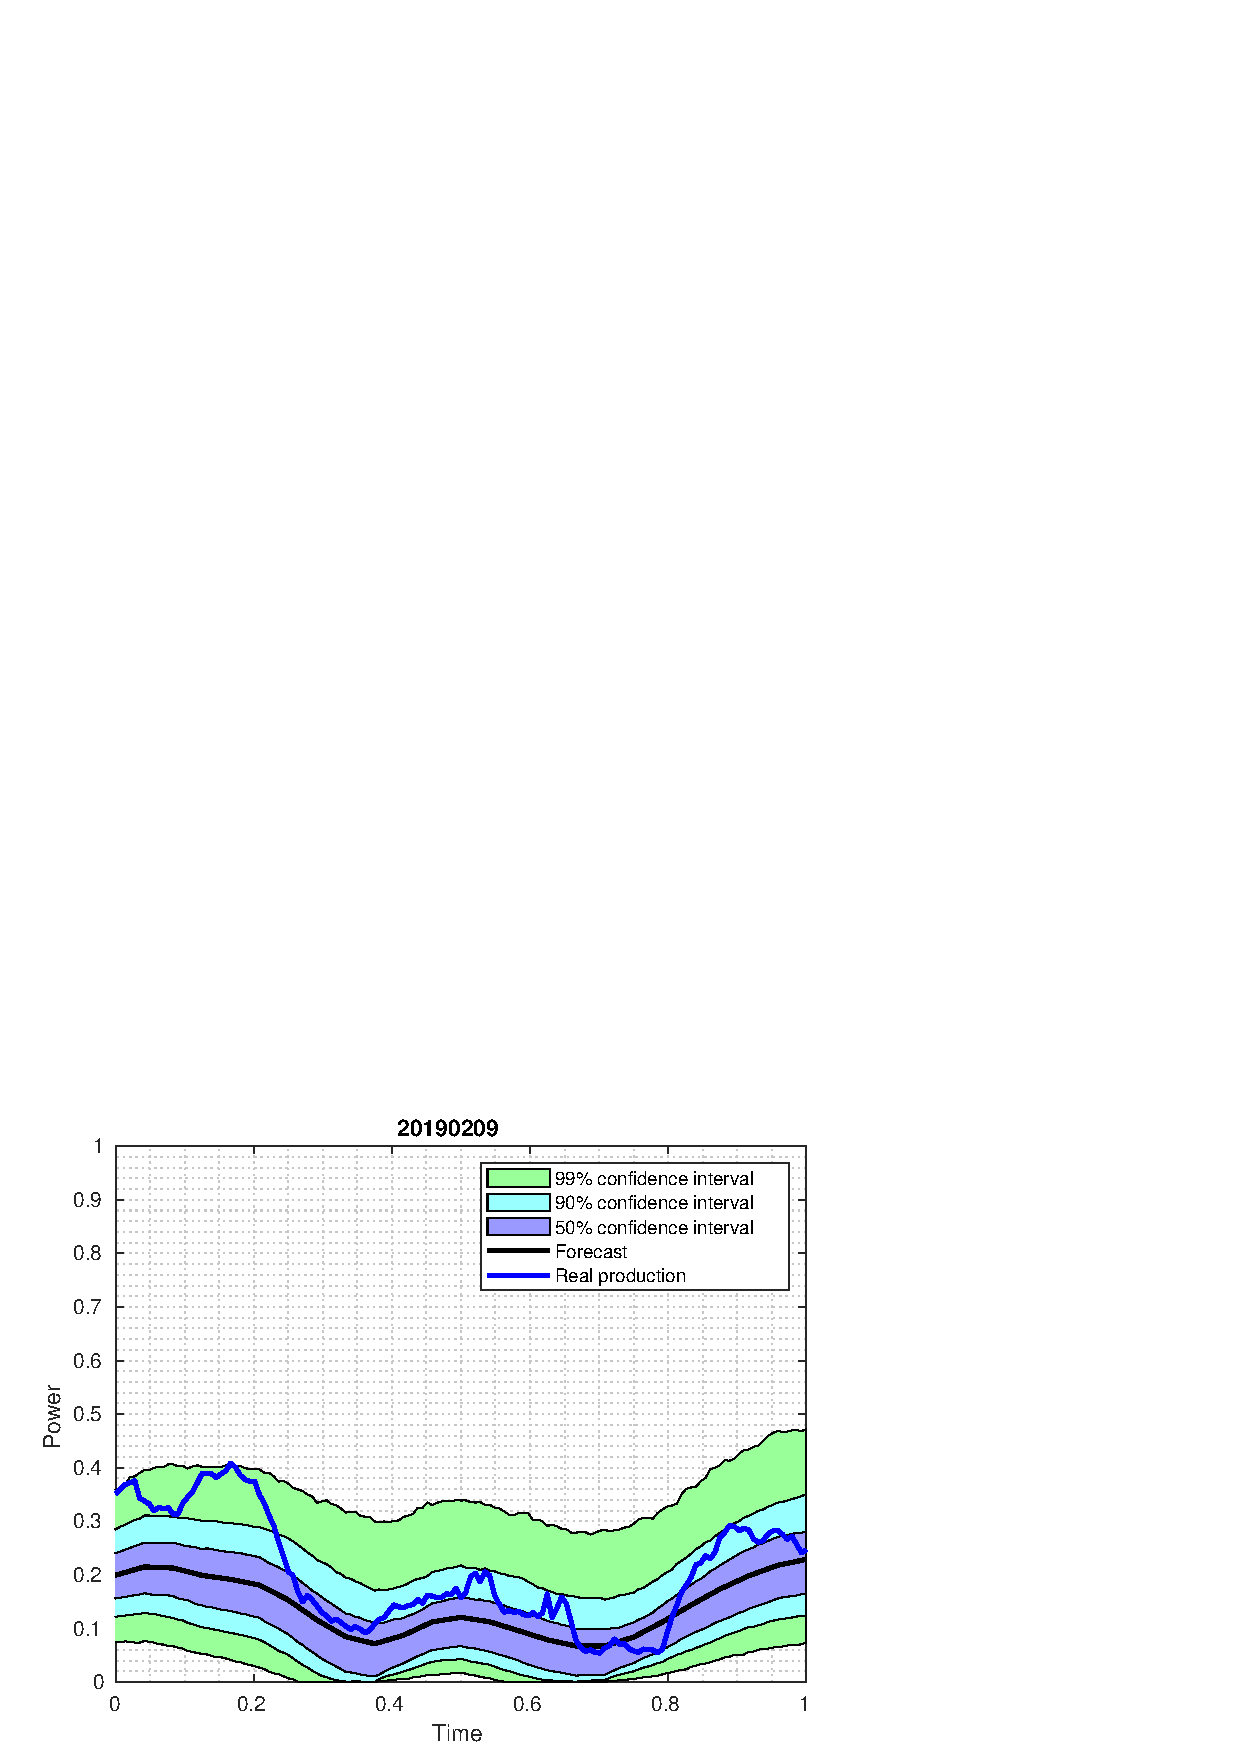
\includegraphics[width=0.8\linewidth]{simulated/24hr/19.pdf}  %DIF > 569
   %DIF > \includegraphics[width=1\linewidth]{simulated/24hr/1099.pdf}
   %DIF > \includegraphics[width=0.9\linewidth]{6hr_forecast_CI_68.pdf}
\end{center}
   \caption{ \DIFaddFL{Examples of simulated paths of wind power production for the next 12 and 24 hours.}}
\label{simulated_24hr}
\end{figure}
\DIFaddend 


\DIFaddbegin \begin{figure}[t]
\begin{center}
%DIF > \fbox{\rule{0pt}{2in} \rule{0.9\linewidth}{0pt}}
  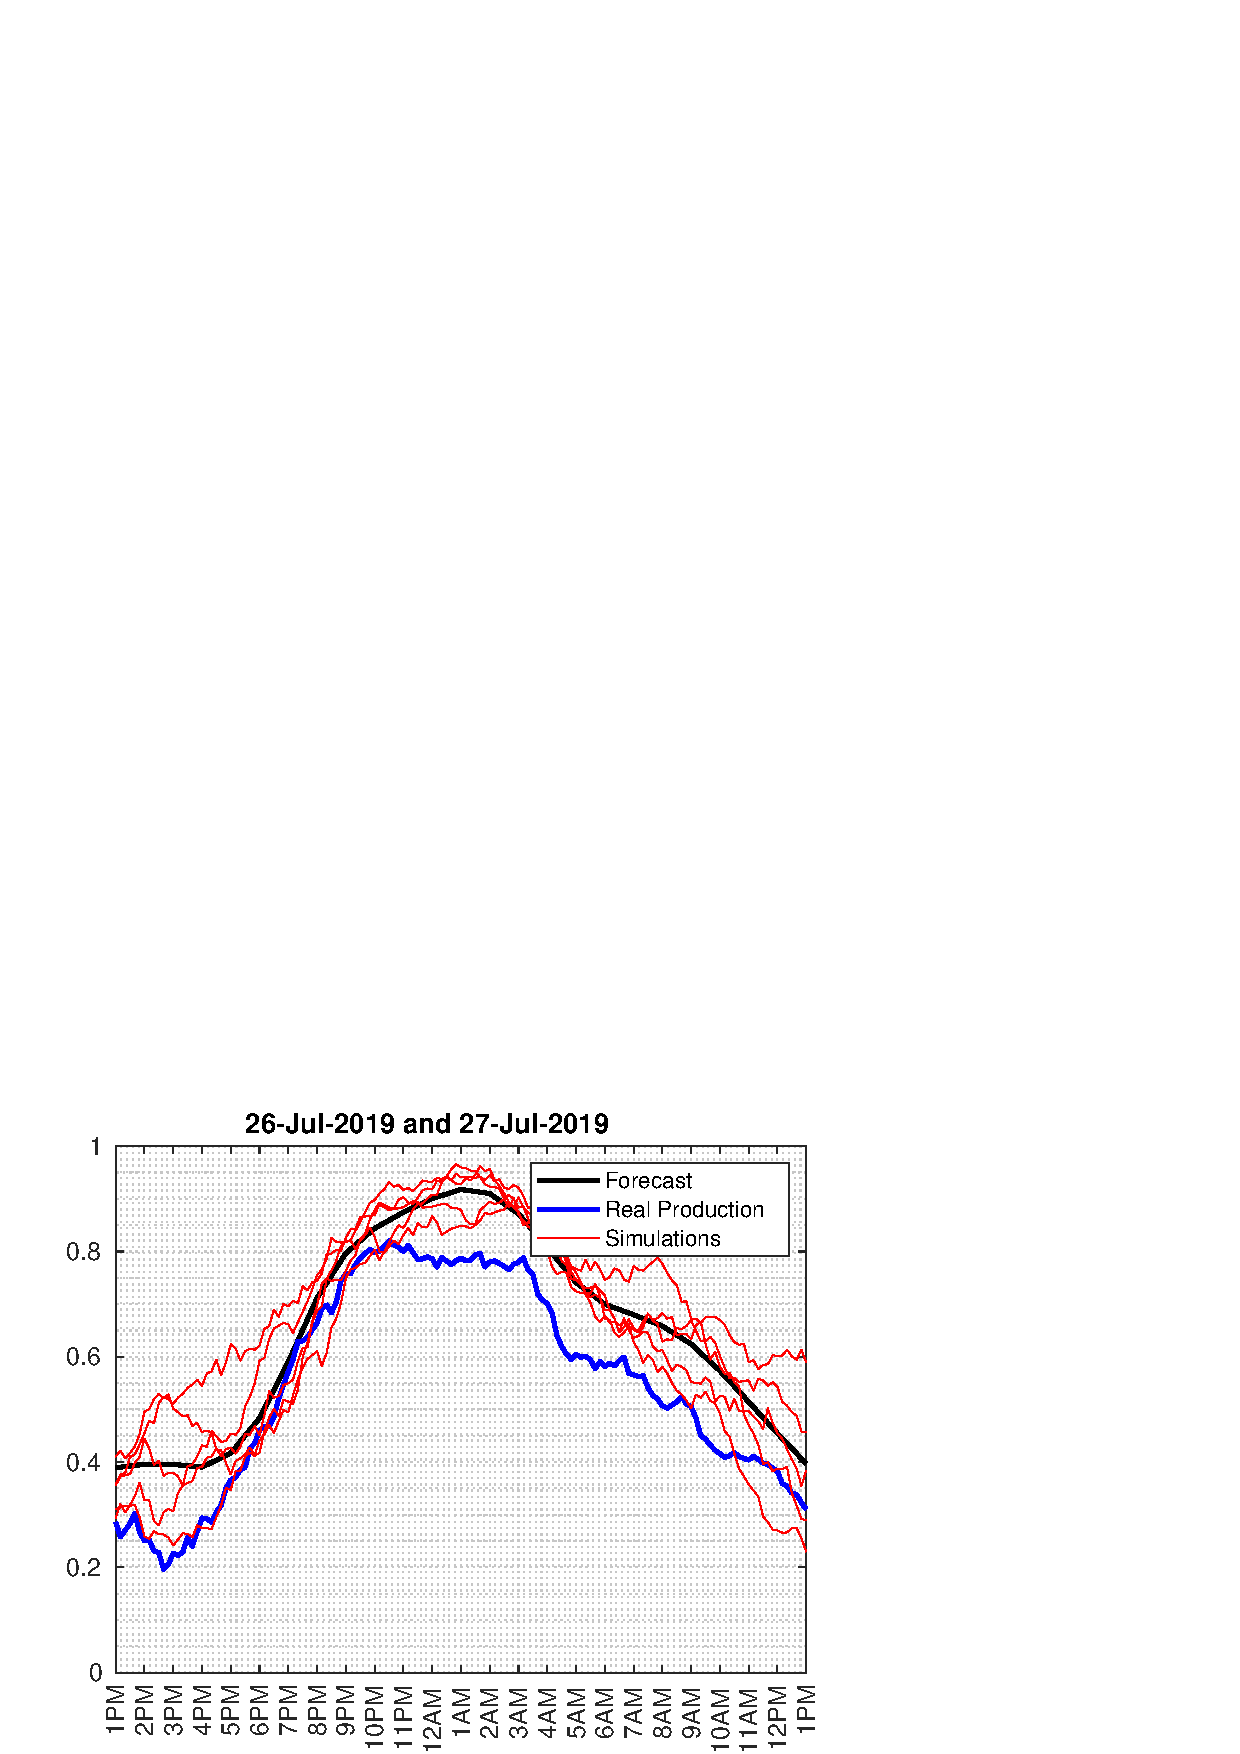
\includegraphics[width=0.8\linewidth]{confidence_intervals/24hr/31.pdf}
  \includegraphics[width=0.8\linewidth]{confidence_intervals/24hr/820.pdf}
  %DIF > 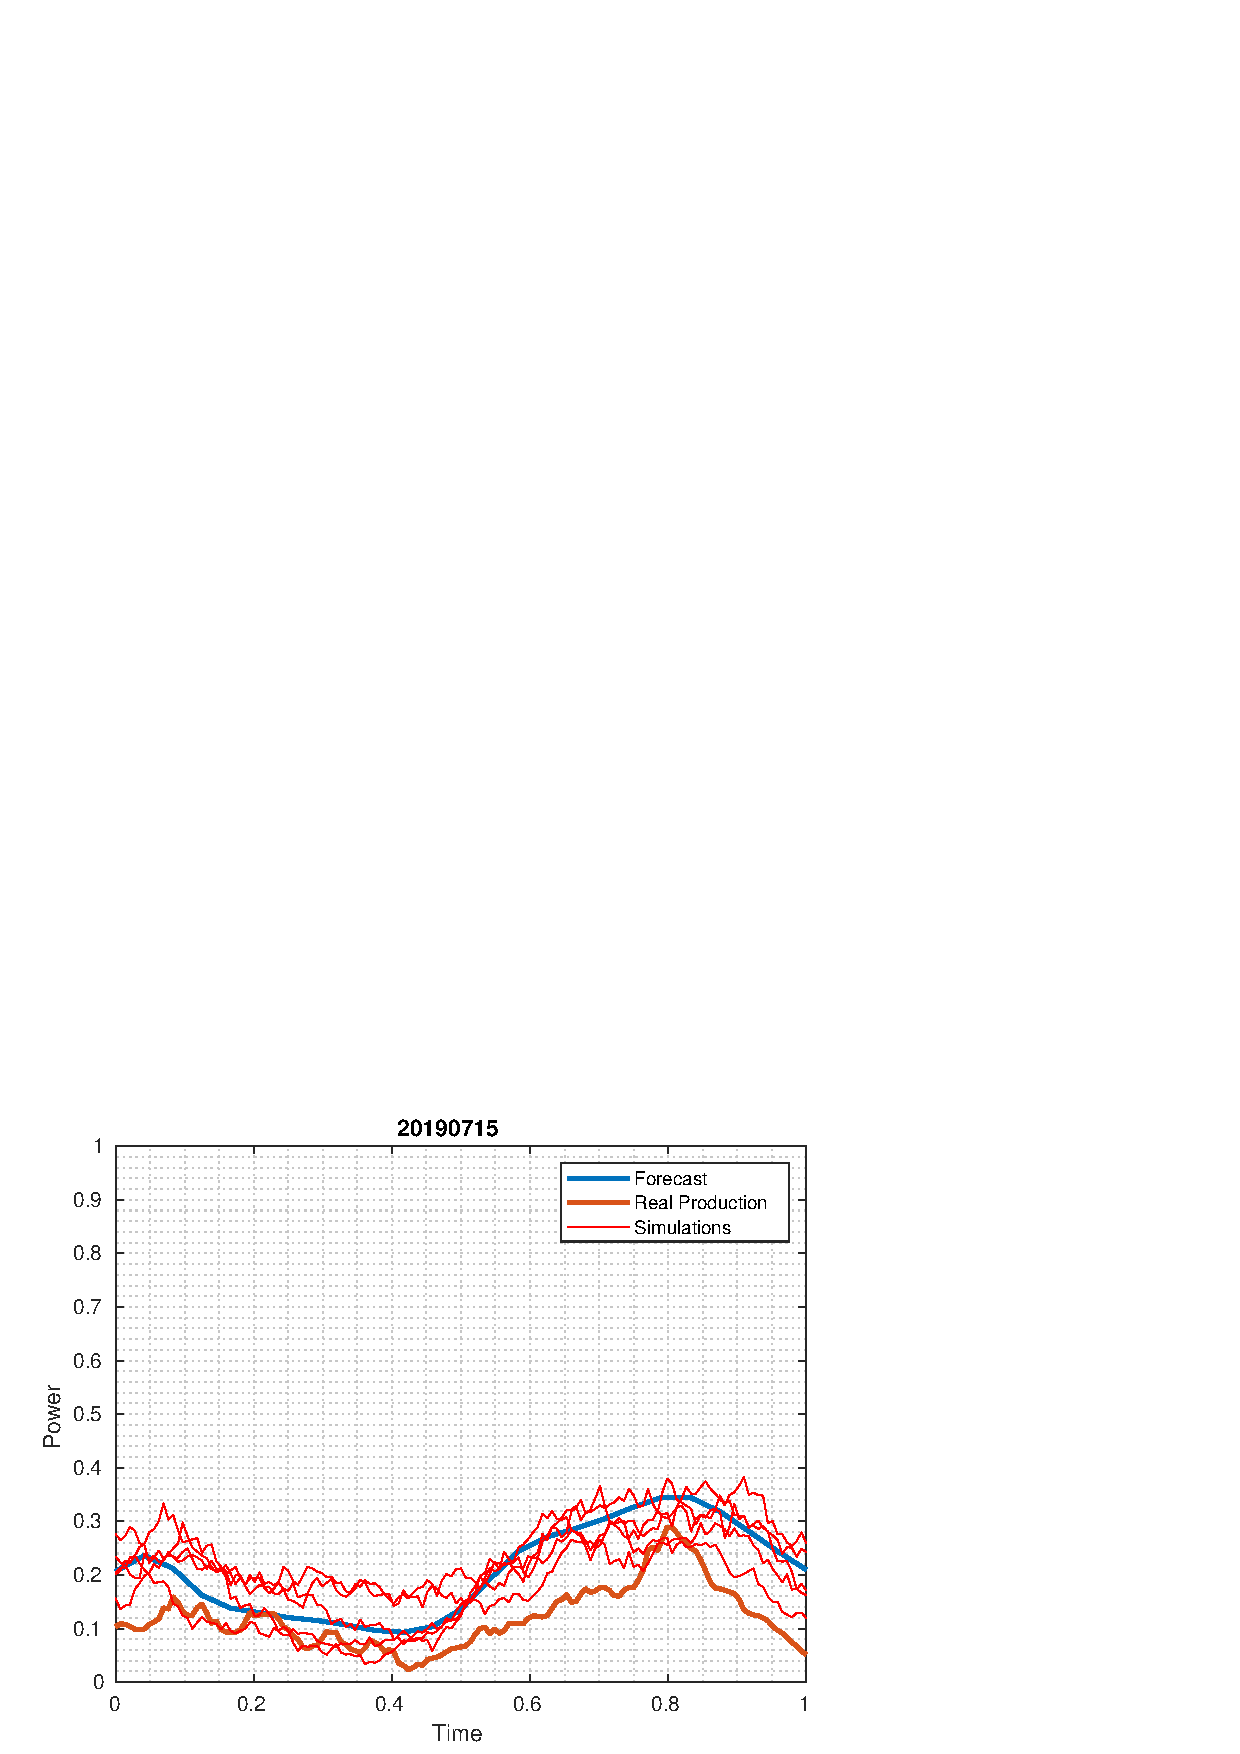
\includegraphics[width=1\linewidth]{confidence_intervals/24hr/82.pdf}

\DIFaddendFL \end{center}
  \caption{ Examples of confidence bands obtained for \DIFdelbeginFL \DIFdelFL{the full 72 }\DIFdelendFL \DIFaddbeginFL \DIFaddFL{24 }\DIFaddendFL hour forecasts. We can see that the model captures the fluctuations in the actual production with non-trivial and asymmetric confidence intervals.}
\label{fig:72hr}
\end{figure}

\begin{figure}[t]
\begin{center}
%\fbox{\rule{0pt}{2in} \rule{0.9\linewidth}{0pt}}
  \DIFdelbeginFL %DIFDELCMD < \includegraphics[width=0.8\linewidth]{6hr_forecast_CI_75.pdf}  %%%
%DIF < 569
   %DIFDELCMD < \includegraphics[width=0.8\linewidth]{6hr_forecast_CI_59.pdf}
%DIFDELCMD <    %%%
\DIFdelendFL \DIFaddbeginFL 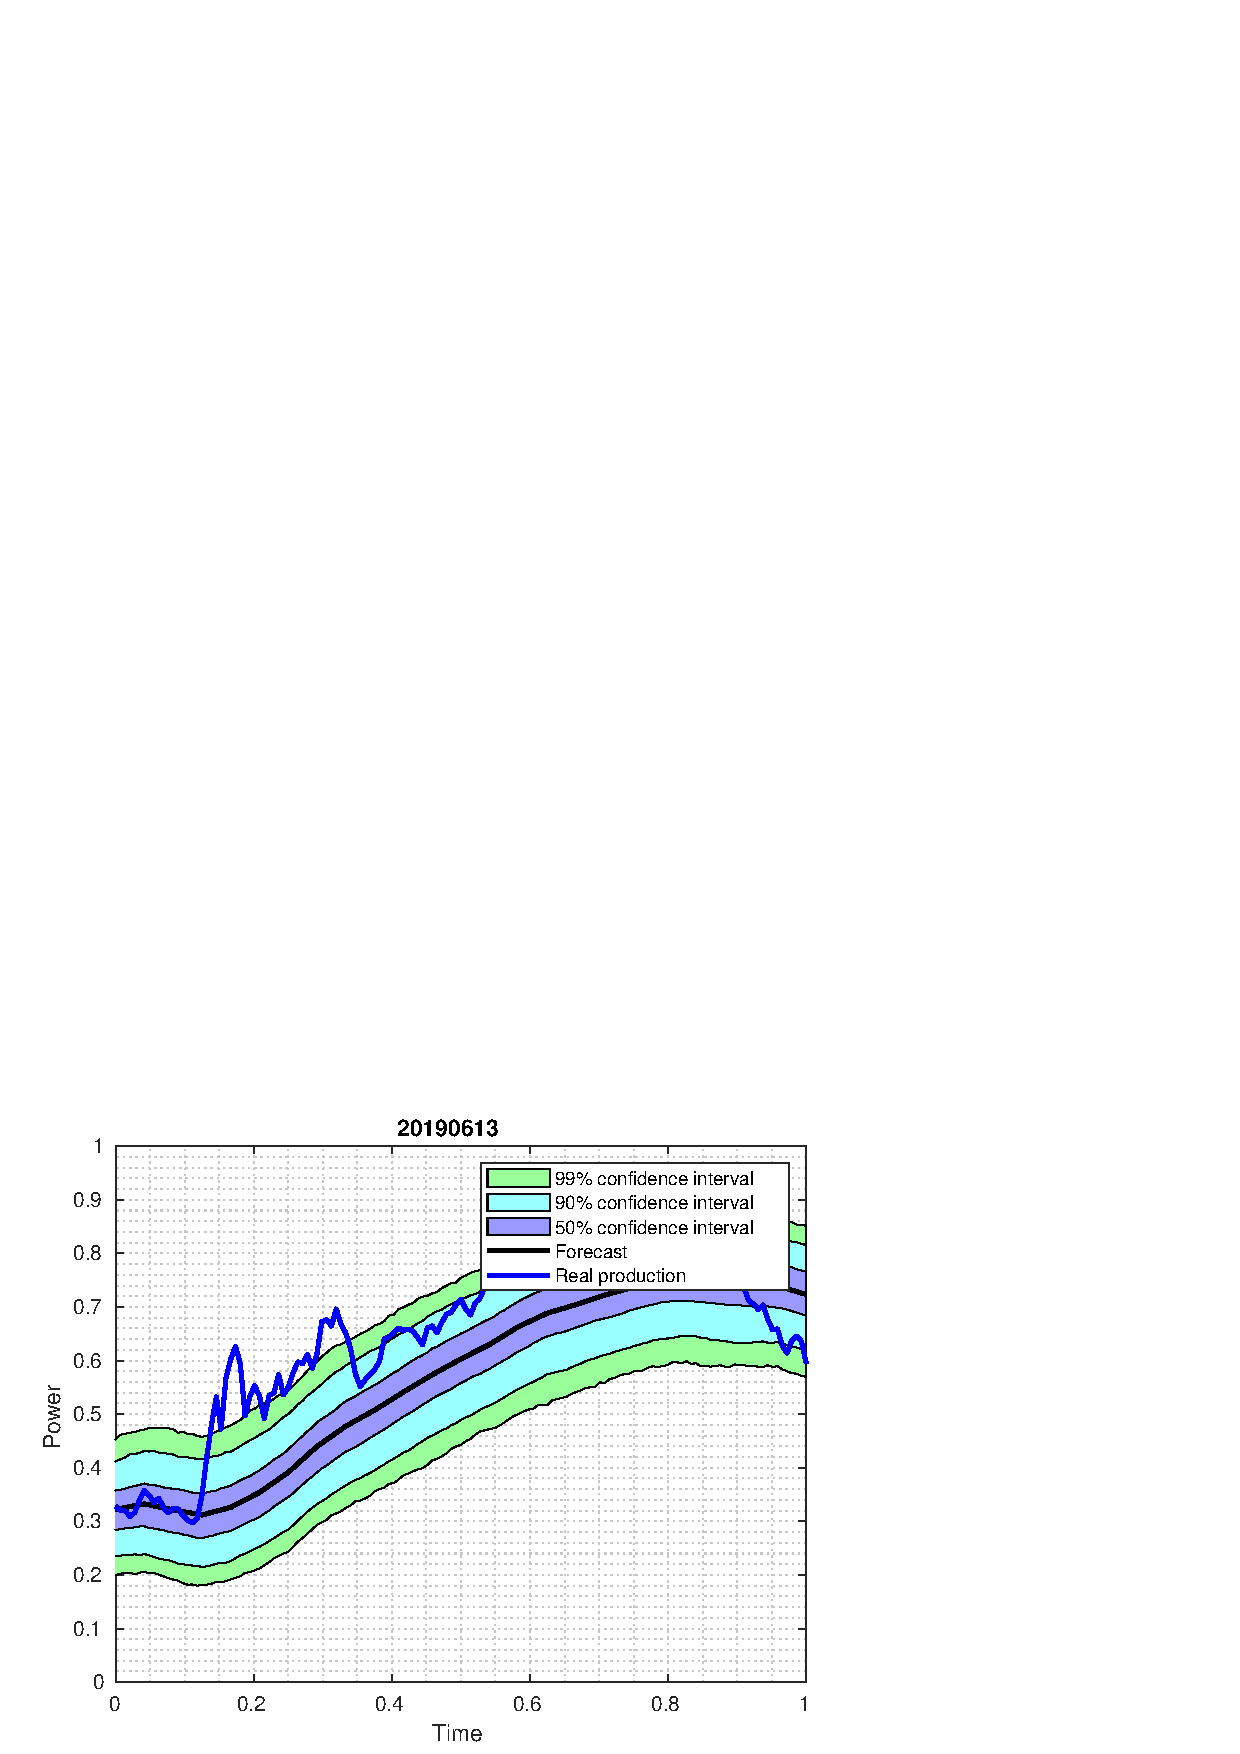
\includegraphics[width=0.8\linewidth]{confidence_intervals/12hr/75.pdf}
  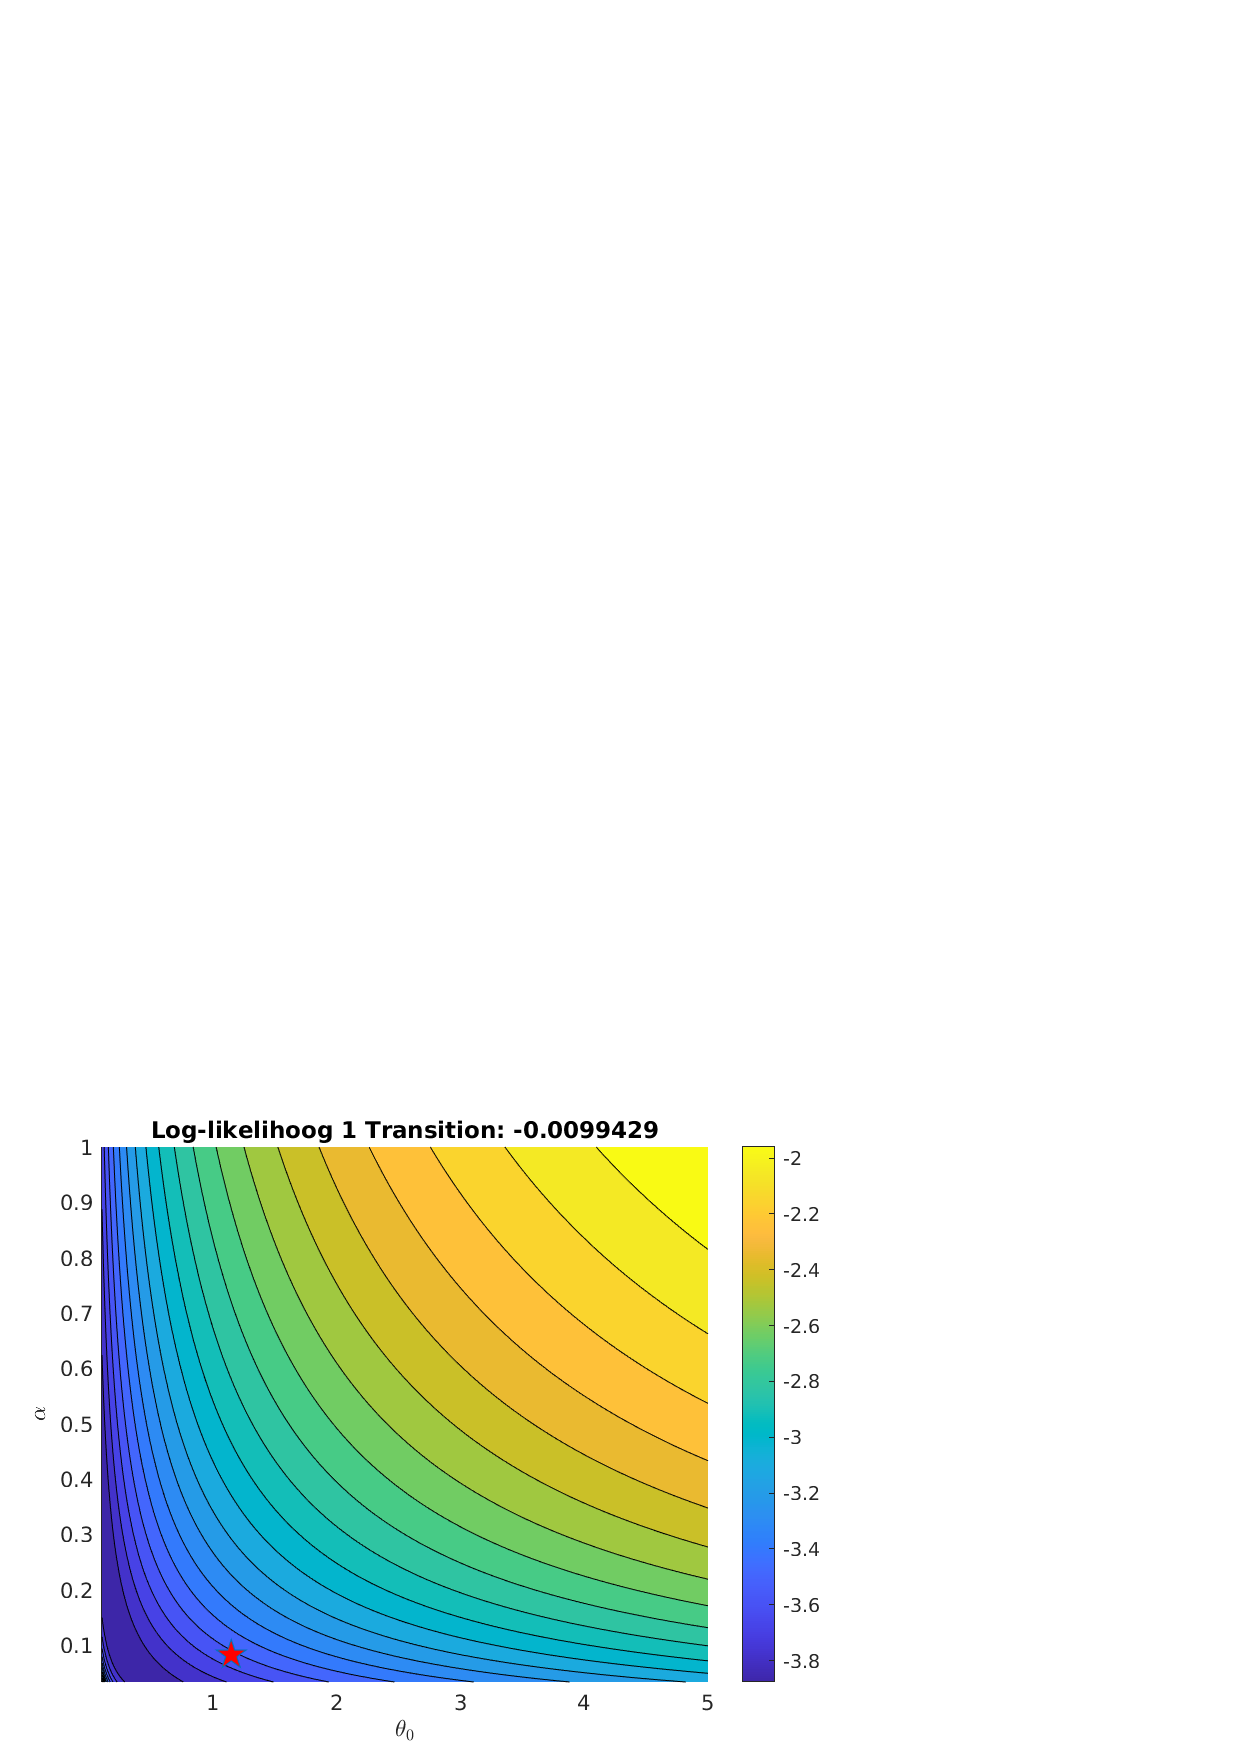
\includegraphics[width=0.8\linewidth]{confidence_intervals/12hr/148.pdf}
  \DIFaddendFL %\includegraphics[width=0.9\linewidth]{6hr_forecast_CI_68.pdf}
\end{center}
  \caption{ Examples of confidence bands obtained for the first \DIFdelbeginFL \DIFdelFL{6 }\DIFdelendFL \DIFaddbeginFL \DIFaddFL{12 }\DIFaddendFL hours of the forecasts. \DIFdelbeginFL \DIFdelFL{This is important as }\DIFdelendFL \DIFaddbeginFL \DIFaddFL{Note that }\DIFaddendFL this \DIFdelbeginFL \DIFdelFL{specific }\DIFdelendFL forecasting company computes a new forecast every \DIFdelbeginFL \DIFdelFL{6 }\DIFdelendFL \DIFaddbeginFL \DIFaddFL{6-9 }\DIFaddendFL hours for reliability.}
\label{fig:6hr}
\end{figure}



 \begin{figure}[t]
\begin{center}
%\fbox{\rule{0pt}{2in} \rule{0.9\linewidth}{0pt}}
   \includegraphics[width=0.8\linewidth]{72hr_forecast_CI_623.pdf}  %569
\end{center}
   \caption{ Examples of omitted data which corresponds to production control and manual energy management decisions. In this example,  wind power production was repeatedly curtailed at around 2 AM which is a period of low power demand. Automatic detection of such scenarios is to be incorporated in future works.}
\label{fig:6hr}
\end{figure}

\section*{Conclusions}
In this project, we have proposed a model based on \DIFdelbegin \DIFdel{SDE's }\DIFdelend \DIFaddbegin \DIFadd{parametric Stochastic Differential Equations and advanced inference }\DIFaddend to quantify uncertainties in wind power generation forecasts. It has the following advantages:
 \begin{itemize} 
\item  Represents and quantifies uncertainty in wind power forecasts \DIFaddbegin \DIFadd{accordingly to their real-world performance}\DIFaddend .
\item \DIFaddbegin \DIFadd{Ability to simulate paths of wind power production.
}\item \DIFaddend It is forecast technology agnostic.
\item  Takes into account physical constrains and the skew-symmetric nature of forecast error.
\item Provides a basis for decision making in the optimal dispatch of electric power.
 \end{itemize} 

%\section*{Acknowledgement}

\DIFdelbegin \section*{\DIFdel{References}}
%DIFAUXCMD
%DIFDELCMD < \begin{flushleft}
%DIFDELCMD < [%%%
\DIFdel{1}%DIFDELCMD < ] {%%%
\DIFdel{Elkantassi, S., Kalligiannaki, E., \& Tempone, R. (2017). Inference And Sensitivity In Stochastic Wind Power Forecast Models. Proceedings of the 2nd International Conference on Uncertainty Quantification in Computational Sciences and Engineering (UNCECOMP 2017). doi:10.7712/120217.5377.16899}%DIFDELCMD < }
%DIFDELCMD < \end{flushleft}
%DIFDELCMD < %%%
\DIFdelend %DIF >  \section*{References}
%DIF >  \begin{flushleft}
%DIF >  [1] {Elkantassi, S., Kalligiannaki, E., \& Tempone, R. (2017). Inference And Sensitivity In Stochastic Wind Power Forecast Models. Proceedings of the 2nd International Conference on Uncertainty Quantification in Computational Sciences and Engineering (UNCECOMP 2017). doi:10.7712/120217.5377.16899}
%DIF >  \end{flushleft}

\end{multicols}
\end{document}
